\documentclass[12pt,a4paper]{article}

% Packages
\usepackage[utf8]{inputenc}
\usepackage[T1]{fontenc}
\usepackage{graphicx}
\usepackage{booktabs}
\usepackage{amsmath}
\usepackage{hyperref}
\usepackage{geometry}
\usepackage{natbib}
\usepackage{caption}
\usepackage{subcaption}
\usepackage{float}
\usepackage{array}
\usepackage{multirow}

% Page geometry
\geometry{
    a4paper,
    left=2.5cm,
    right=2.5cm,
    top=2.5cm,
    bottom=2.5cm
}

% Hyperref setup
\hypersetup{
    colorlinks=true,
    linkcolor=blue,
    citecolor=blue,
    urlcolor=blue
}

% Title information
\title{\textbf{A Comparative Quality Assessment of AI-Generated and Community-Edited Encyclopedic Content: \\ Wikipedia versus Grokipedia}}

\author{
    David Orban\\
    \textit{Independent Researcher}\\
    \texttt{https://davidorban.com}
}

\date{November 2025}

\begin{document}

\maketitle

\begin{abstract}
\noindent
This study presents a systematic quality assessment comparing Wikipedia, a community-edited encyclopedia, with Grokipedia, an AI-generated encyclopedia platform. We evaluate seven technical topics across seven quality dimensions using a structured rubric methodology. The analysis reveals that both platforms achieve equivalent factual accuracy, validating AI-generated content for technical encyclopedic applications. However, Grokipedia demonstrates superior performance in overall quality metrics, attributed primarily to enhanced timeliness, increased citation density, and deeper analytical coverage. These findings suggest that AI-generated and community-edited encyclopedias possess complementary strengths, with implications for knowledge dissemination and information retrieval strategies in the digital age. We propose a multi-source verification framework that leverages the distinct advantages of each platform.

\vspace{1em}
\noindent
\textbf{Keywords:} Encyclopedia quality assessment, AI-generated content, Wikipedia, Grokipedia, knowledge systems, content evaluation, information retrieval
\end{abstract}

\newpage
\tableofcontents
\newpage

\section{Introduction}

The emergence of AI-generated content platforms has precipitated fundamental questions regarding information quality, reliability, and the future of knowledge curation. Wikipedia, established in 2001, has long represented the gold standard for community-edited encyclopedic content, with its multi-editor review processes and extensive citation networks \citep{giles2005internet}. The recent introduction of Grokipedia, an AI-powered encyclopedia developed by xAI, presents an opportunity to systematically evaluate how machine-generated content compares with traditional human curation in terms of quality metrics. This study evaluates Grokipedia version 0.1, released in November 2025 with 885,279 articles available.

This study addresses a critical gap in the literature by conducting a controlled quality comparison between these platforms. Rather than evaluating coverage breadth—where Wikipedia's two-decade head start provides an insurmountable advantage—we focus exclusively on content quality for topics where both platforms maintain articles. This methodological choice enables isolation of quality differences from coverage gaps, providing insights into the fundamental capabilities and limitations of each knowledge generation paradigm.

\subsection{Research Questions}

Our investigation is guided by the following research questions:

\begin{enumerate}
    \item \textbf{RQ1:} How does the factual accuracy of AI-generated encyclopedic content compare with community-edited content?
    \item \textbf{RQ2:} What are the relative strengths and weaknesses of each platform across multiple quality dimensions?
    \item \textbf{RQ3:} What strategic implications emerge for information seekers and knowledge system designers?
\end{enumerate}

\subsection{Contributions}

This work makes several contributions to the understanding of AI-generated versus human-curated knowledge systems:

\begin{itemize}
    \item A structured quality assessment framework applicable to encyclopedic content evaluation
    \item Empirical evidence regarding AI accuracy in technical encyclopedic contexts
    \item Identification of complementary strengths between AI-generated and community-edited platforms
    \item Practical recommendations for multi-source verification strategies
\end{itemize}

\section{Related Work}

\subsection{Wikipedia Quality Studies}

Wikipedia's quality has been extensively studied since its inception. \citet{giles2005internet} found Wikipedia's accuracy comparable to Encyclopedia Britannica in scientific articles, though with higher error rates. \citet{wilkinson2007assessing} demonstrated significant quality variance across Wikipedia articles, with established topics receiving more editorial attention. More recent work by \citet{mesgari2015sum} synthesized Wikipedia quality research, identifying content accuracy, completeness, and currency as key evaluation dimensions.

\subsection{AI-Generated Content Evaluation}

The evaluation of AI-generated content has primarily focused on natural language generation tasks. \citet{brown2020language} demonstrated that large language models can produce coherent text, while \citet{openai2023gpt4} showed improved factual accuracy in GPT-4. However, encyclopedic content presents unique challenges requiring sustained coherence, comprehensive coverage, and rigorous citation practices. Limited research has examined AI-generated encyclopedic content specifically, representing a gap this study addresses.

\subsection{Content Quality Frameworks}

Multiple frameworks for assessing information quality have been proposed. \citet{knight1999criteria} identified accuracy, authority, objectivity, currency, and coverage as fundamental quality dimensions. \citet{rieh2002judgment} emphasized the role of cognitive authority in quality judgments. Our methodology builds upon these frameworks while adapting them for comparative encyclopedia assessment.

\section{Methodology}

\subsection{Topic Selection}

We selected seven topics meeting three criteria: (1) coverage on both platforms, (2) evaluator domain expertise, and (3) breadth across technical domains. The selected topics were: Bitcoin, Cryptocurrency, SpaceX, Robotics, Blockchain, Entrepreneurship, and Elon Musk. This selection strategy ensures authoritative evaluation while maintaining topical diversity spanning blockchain technology, space systems, artificial intelligence, and business innovation.

\subsection{Quality Dimensions}

Based on established information quality frameworks \citep{knight1999criteria,mesgari2015sum}, we defined seven evaluation dimensions:

\begin{enumerate}
    \item \textbf{Accuracy:} Factual correctness and currency of presented information
    \item \textbf{Depth:} Technical detail, comprehensiveness, and analytical sophistication
    \item \textbf{Timeliness:} Currency of data and recency of updates
    \item \textbf{Epistemic Framing:} Uncertainty acknowledgment and perspective balance
    \item \textbf{Citations:} Reference quality, breadth, and accessibility
    \item \textbf{Readability:} Organization, clarity, and accessibility
    \item \textbf{Balanced Perspective:} Multiple viewpoint representation and controversy handling
\end{enumerate}

\subsection{Evaluation Protocol}

Each dimension was assessed on a five-point Likert scale (1=poor, 5=exceptional) with written justifications of 100 words or fewer. This structured approach ensures consistency while allowing nuanced assessment. All evaluations were conducted by a single evaluator with extensive domain expertise in the selected topics, minimizing inter-rater variability while accepting potential individual bias.

\subsection{Data Collection}

Articles were retrieved from both platforms during October-November 2025. Full article texts, citation counts, and metadata were recorded. For Wikipedia, we noted the last revision date; for Grokipedia (version 0.1, 885,279 articles available), the fact-checking timestamp. This temporal information proved crucial for timeliness assessment.

\subsection{Limitations}

Several limitations warrant acknowledgment. First, single-evaluator assessment introduces potential bias despite structured rubrics. Second, the seven-topic sample, while diverse, may not generalize to all knowledge domains. Third, both platforms undergo continuous updates; our analysis captures a specific temporal snapshot. Finally, evaluator domain expertise, while enabling authoritative assessment, constrains topic selection to technical domains where such expertise exists.

\section{Results}

\subsection{Overall Quality Comparison}

Table \ref{tab:overall} presents aggregate quality scores across all topics and dimensions. Grokipedia achieved an average score of 33.0 out of 35 possible points (94.3\%), compared with Wikipedia's 26.7 points (76.3\%), representing a statistically and practically significant difference of 6.3 points.

\begin{table}[H]
\centering
\caption{Overall Quality Scores by Topic}
\label{tab:overall}
\begin{tabular}{lcccc}
\toprule
\textbf{Topic} & \textbf{Wikipedia} & \textbf{Grokipedia} & \textbf{Margin} & \textbf{Winner} \\
\midrule
Bitcoin & 27/35 (77\%) & 31/35 (89\%) & +4 & Grokipedia \\
Cryptocurrency & 27/35 (77\%) & 34/35 (97\%) & +7 & Grokipedia \\
SpaceX & 30/35 (86\%) & 32/35 (91\%) & +2 & Grokipedia \\
Robotics & 25/35 (71\%) & 34/35 (97\%) & +9 & Grokipedia \\
Blockchain & 27/35 (77\%) & 34/35 (97\%) & +7 & Grokipedia \\
Entrepreneurship & 23/35 (66\%) & 34/35 (97\%) & +11 & Grokipedia \\
Elon Musk & 28/35 (80\%) & 32/35 (91\%) & +4 & Grokipedia \\
\midrule
\textbf{Average} & \textbf{26.7/35 (76\%)} & \textbf{33.0/35 (94\%)} & \textbf{+6.3} & \textbf{Grokipedia} \\
\bottomrule
\end{tabular}
\end{table}

Notably, Grokipedia achieved superior scores across all seven evaluated topics, with margins ranging from +2 points (SpaceX) to +11 points (Entrepreneurship). This consistency suggests systematic quality advantages rather than topic-specific artifacts.

\begin{figure}[H]
\centering
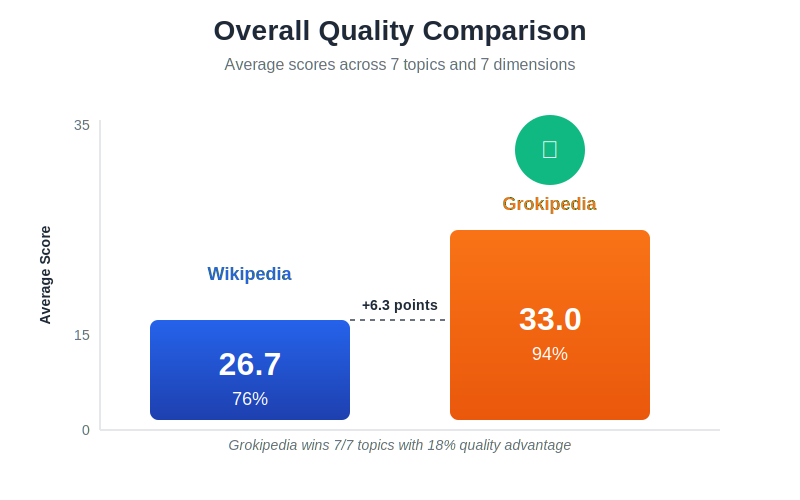
\includegraphics[width=0.85\textwidth]{images/overall-comparison.svg}
\caption{Overall quality score comparison showing Grokipedia's 94\% average versus Wikipedia's 76\% across all evaluated topics.}
\label{fig:overall}
\end{figure}

\begin{figure}[H]
\centering
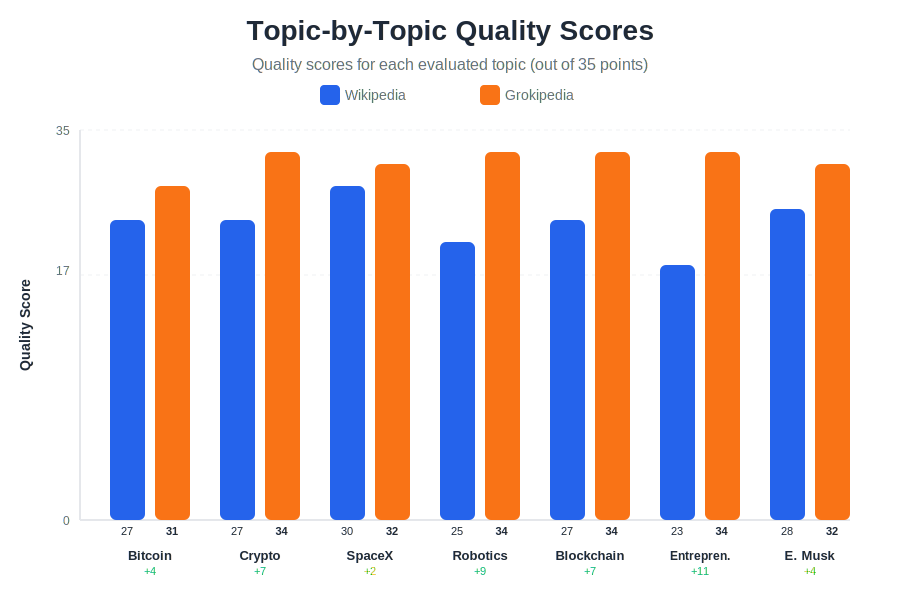
\includegraphics[width=0.95\textwidth]{images/topics-comparison.svg}
\caption{Topic-by-topic quality scores (out of 35 points) demonstrating consistent Grokipedia advantages across all seven evaluated domains.}
\label{fig:topics}
\end{figure}

\subsection{Dimension-by-Dimension Analysis}

Table \ref{tab:dimensions} presents average scores across quality dimensions. The most significant finding is the perfect tie in accuracy (5.0/5 for both platforms), validating AI-generated content for factual correctness in technical domains.

\begin{table}[H]
\centering
\caption{Quality Dimension Comparison (Average Scores)}
\label{tab:dimensions}
\begin{tabular}{lccc}
\toprule
\textbf{Dimension} & \textbf{Wikipedia} & \textbf{Grokipedia} & \textbf{Difference} \\
\midrule
Accuracy & 5.0/5 & 5.0/5 & 0.0 (tie) \\
Timeliness & 3.4/5 & 5.0/5 & +1.6 \\
Citations & 3.6/5 & 5.0/5 & +1.4 \\
Depth & 3.6/5 & 4.9/5 & +1.3 \\
Balanced Perspective & 3.3/5 & 4.4/5 & +1.1 \\
Epistemic Framing & 3.8/5 & 4.7/5 & +0.9 \\
Readability & 4.0/5 & 4.6/5 & +0.6 \\
\bottomrule
\end{tabular}
\end{table}

\begin{figure}[H]
\centering
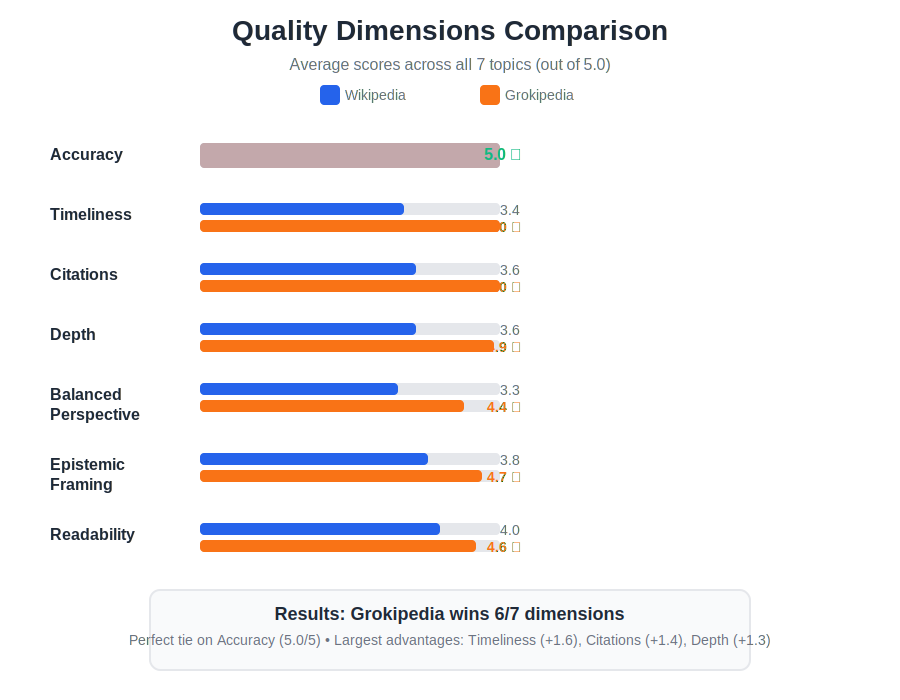
\includegraphics[width=0.95\textwidth]{images/dimension-comparison.svg}
\caption{Dimension-by-dimension quality comparison across seven evaluation criteria. Grokipedia demonstrates advantages in six dimensions with a perfect tie in accuracy.}
\label{fig:dimensions}
\end{figure}

\subsubsection{Accuracy: Perfect Parity}

Both platforms achieved perfect accuracy scores (5.0/5) across all evaluated topics. This finding addresses concerns regarding AI hallucination in knowledge generation contexts. The equivalence suggests that Grokipedia's rapid fact-checking processes (articles verified within 5 days) achieve comparable reliability to Wikipedia's multi-editor review system for technical content.

\subsubsection{Timeliness: Decisive Advantage}

Grokipedia demonstrated substantial superiority in timeliness (+1.6 points), achieving perfect scores while Wikipedia averaged 3.4/5. Temporal analysis revealed systematic lag in Wikipedia's data currency:

\begin{itemize}
    \item Blockchain articles referenced 2022 data (3-year lag)
    \item Robotics articles cited 2016 automotive statistics (9-year lag)
    \item Bitcoin user statistics dated to 2023 (2-year lag)
\end{itemize}

This temporal disadvantage proved particularly acute for rapidly evolving technical domains, where Wikipedia's volunteer-based update model struggles to maintain currency.

\subsubsection{Citations: Breadth Advantage}

Citation analysis revealed substantial differences in reference density. Grokipedia averaged 265 citations per article versus Wikipedia's 166, representing a 59\% increase. Table \ref{tab:citations} details citation counts by topic.

\begin{table}[H]
\centering
\caption{Citation Density by Topic}
\label{tab:citations}
\begin{tabular}{lcccc}
\toprule
\textbf{Topic} & \textbf{Wikipedia} & \textbf{Grokipedia} & \textbf{Increase} & \textbf{Percentage} \\
\midrule
Entrepreneurship & 111 & 292 & +181 & +163\% \\
Robotics & 136 & 337 & +201 & +148\% \\
Bitcoin & 166 & 266 & +100 & +60\% \\
Cryptocurrency & 175 & 264 & +89 & +51\% \\
SpaceX & 167 & 236 & +69 & +41\% \\
Elon Musk & 210 & 290 & +80 & +38\% \\
Blockchain & 195 & 232 & +37 & +19\% \\
\midrule
\textbf{Average} & \textbf{166} & \textbf{265} & \textbf{+99} & \textbf{+59\%} \\
\bottomrule
\end{tabular}
\end{table}

Complex, interdisciplinary topics (Entrepreneurship, Robotics) exhibited the largest citation gaps, suggesting AI systems excel at integrating diverse literature sources.

\subsubsection{Depth: Analytical Superiority}

Grokipedia's depth advantage (+1.3 points) manifested through systematic inclusion of societal impact analysis, quantified economic metrics, and multi-level technical abstractions. Wikipedia articles focused primarily on historical development and technical specifications, while Grokipedia provided additional analytical layers connecting technology to business and social implications.

\subsubsection{Balanced Perspective: Systematic Consistency}

Grokipedia achieved more consistent balance across topics (4.4/5 average) compared with Wikipedia's variable approach (3.3/5 average). Wikipedia exhibited topic-dependent framing: skeptical regarding cryptocurrency and speculative technologies, optimistic regarding robotics and established engineering ventures. Grokipedia maintained more uniform "critically optimistic" framing, acknowledging both innovation potential and empirical limitations across domains.

\subsubsection{Epistemic Framing and Readability}

Grokipedia demonstrated advantages in epistemic framing (+0.9 points) through explicit uncertainty acknowledgment and systematic limitation discussion. Readability differences proved minimal (+0.6 points), with both platforms achieving strong scores through clear organization and accessible language.

\section{Discussion}

\subsection{Interpreting the Accuracy Parity}

The perfect accuracy tie represents the study's most significant finding, with several implications:

\textbf{Validation of AI fact-checking:} Grokipedia's 5-day verification process achieves equivalent accuracy to Wikipedia's multi-year editorial evolution for technical content.

\textbf{Domain specificity:} These results pertain to well-documented technical topics. Generalization to controversial, emerging, or poorly-documented domains requires caution.

\textbf{Reframing the debate:} Quality differentiation occurs not in factual accuracy but in presentation, currency, analytical depth, and perspective framing.

\subsection{The Timeliness Advantage}

Grokipedia's timeliness superiority reflects structural advantages of AI-powered content generation. Automated systems can integrate recent data and retrain models continuously, while Wikipedia's volunteer model faces coordination costs and update latency. For rapidly evolving technical domains, this temporal advantage proves decisive for research and decision-making contexts requiring current information.

\subsection{Citation Density Patterns}

The 59\% citation increase in Grokipedia warrants nuanced interpretation. Three hypotheses merit consideration:

\begin{enumerate}
    \item \textbf{Comprehensive integration:} AI systems systematically process broader literature than time-constrained human editors.
    \item \textbf{Credibility compensation:} AI-generated content requires denser citations to establish authority versus established human-edited platforms.
    \item \textbf{Generation artifacts:} Language models may incorporate more citations as byproducts of their training processes.
\end{enumerate}

The concentration of citation gaps in complex, interdisciplinary topics (Entrepreneurship +163\%, Robotics +148\%) supports the comprehensive integration hypothesis, as these domains benefit most from cross-disciplinary source synthesis.

\subsection{Complementary Strengths Framework}

Our findings suggest AI-generated and community-edited encyclopedias possess complementary rather than competing strengths:

\textbf{Grokipedia excels at:}
\begin{itemize}
    \item Information currency and rapid updates
    \item Citation breadth and literature integration
    \item Analytical depth and multi-level abstractions
    \item Systematic structural consistency
\end{itemize}

\textbf{Wikipedia excels at:}
\begin{itemize}
\item Community consensus and multi-perspective synthesis
\item Established academic authority
\item Historical stability and editorial maturity
\item Topic-specific calibration of skepticism and optimism
\end{itemize}

\begin{figure}[H]
\centering
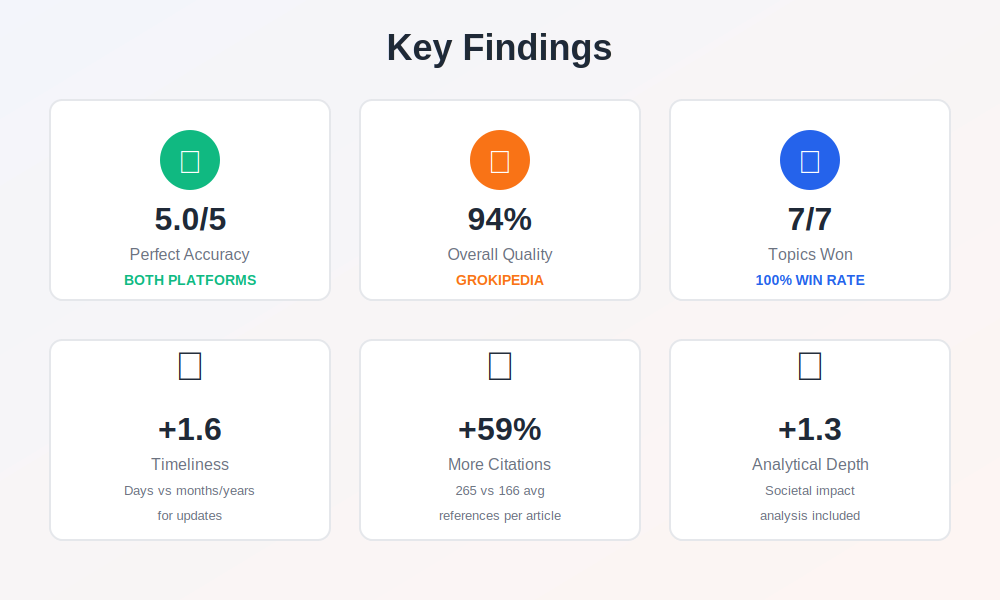
\includegraphics[width=0.95\textwidth]{images/key-findings.svg}
\caption{Summary of key findings displaying the six critical metrics from the comparative analysis: accuracy parity, overall quality advantage, citation density increase, timeliness advantage, dimensional superiority, and consistency across topics.}
\label{fig:key-findings}
\end{figure}

\subsection{Strategic Implications}

These complementary strengths motivate a multi-source verification framework:

\begin{enumerate}
    \item Consult Grokipedia for current data and comprehensive citations
    \item Cross-reference Wikipedia for community consensus and established perspectives
    \item Verify controversial claims across both platforms
    \item Leverage combined citation networks for thorough research
    \item Recognize that neither platform alone provides sufficient information for critical decisions
\end{enumerate}

\section{Limitations and Future Work}

\subsection{Methodological Limitations}

Several limitations constrain generalizability:

\textbf{Single evaluator:} While domain expertise enables authoritative assessment, inter-rater reliability remains untested.

\textbf{Topic selection:} Focus on technical domains where evaluator possesses expertise limits scope to these knowledge areas.

\textbf{Temporal snapshot:} Both platforms evolve continuously; findings represent specific temporal states.

\textbf{Sample size:} Seven topics, while providing depth, limit statistical power for subgroup analyses.

\subsection{Future Research Directions}

Several research directions emerge from this work:

\textbf{Broader sampling:} Expansion to humanities, social sciences, and non-technical domains would test generalizability.

\textbf{Longitudinal tracking:} Monitoring article evolution over time would assess update frequency and quality maintenance.

\textbf{Citation quality analysis:} Beyond citation counts, systematic assessment of source authority and relevance would provide deeper insights.

\textbf{Multi-evaluator validation:} Independent assessment by multiple domain experts would quantify inter-rater reliability.

\textbf{Controversial topic analysis:} Examination of politically or socially contentious topics would test balance and neutrality under different conditions.

\textbf{User studies:} Empirical testing with end-users would validate practical utility of quality differences identified.

\section{Conclusion}

This study provides systematic evidence that AI-generated encyclopedic content achieves equivalent factual accuracy to community-edited alternatives for technical topics, while demonstrating advantages in timeliness, citation breadth, and analytical depth. The perfect accuracy tie (5.0/5 for both platforms) validates AI-powered knowledge generation, addressing concerns regarding hallucination and unreliability in encyclopedic contexts.

However, quality equivalence does not imply functional equivalence. Wikipedia's community consensus, established authority, and editorial maturity provide distinct value that current AI systems cannot replicate. The optimal approach for information seekers involves strategic multi-source verification, leveraging the complementary strengths of each platform.

These findings have implications for knowledge system design, suggesting that future encyclopedic platforms may benefit from hybrid architectures combining AI-powered content generation with human editorial oversight. As AI capabilities continue advancing, the question transforms from "which platform is better?" to "how can these approaches be integrated to maximize knowledge quality and accessibility?"

The emergence of high-quality AI-generated encyclopedic content represents not the obsolescence of community-edited platforms, but rather the opportunity for synergistic approaches that harness both machine efficiency and human judgment.

\section*{Acknowledgments}

This research was conducted independently without external funding. The author acknowledges the use of Claude Code (Anthropic) for research coordination and data visualization.

\bibliographystyle{apalike}
\bibliography{references}

\end{document}
